\chapter{Methodology}
\label{ch:methodology}

This chapter presents the methodological framework adopted in this thesis for comparing PageRank and HITS on a real-world football transfer network. The methodology combines formal graph modeling, distributed data processing using PySpark, algorithm implementation, experimental design, and the development of an interactive web-based analysis environment. The chapter proceeds from the abstract problem formulation to the concrete implementation of the \textit{Transfer Analyzer} system and the experimental protocol used to interpret the obtained rankings.


%=============================================================
\section{Problem Formulation}
\label{sec:problem_formulation}

The central objective of this thesis is to compare the behavior of PageRank and HITS when applied to the same weighted directed network under controlled and configurable conditions. The selected application domain is the professional football transfer market, in which clubs exchange players across leagues and seasons for monetary transfer fees.

\begin{definition}[Football Transfer Network]
The football transfer network is modeled as a weighted directed graph
\[
G = (V, E, W),
\]
where:
\begin{itemize}
    \item $V$ is the set of football clubs;
    \item $E \subseteq V \times V$ is the set of directed edges such that an edge $(u,v)$ exists if club $u$ transferred at least one player to club $v$;
    \item $W: E \rightarrow \mathbb{R}^{+}$ is a weight function assigning a non-negative value to each edge.
\end{itemize}
\end{definition}

In the context of this thesis, the direction of each edge is defined from the \textit{selling club} to the \textit{buying club}. This choice preserves the economic meaning of transfer flow: talent and market value move from source club to destination club.

Two edge-weighting schemes are considered:
\begin{enumerate}
    \item \textbf{Fee-weighted mode:} the weight of an edge is the total transfer fee aggregated across all transfers between the same ordered pair of clubs.
    \item \textbf{Count-weighted mode:} the weight of an edge is the number of transfer events between the same ordered pair of clubs.
\end{enumerate}

The problem addressed by this thesis may therefore be stated as follows: given a filtered football transfer graph $G'$, compute and compare the rankings produced by PageRank and HITS, analyze how the rankings vary under changes in weighting mode and filtering conditions, and provide interactive visual evidence that supports the interpretation of each algorithm's output.


%=============================================================
\section{Distributed Graph Processing Pipeline}
\label{sec:pipeline}

The computational pipeline transforms raw transfer records into algorithm-ready graph structures and then into visualization-ready ranking outputs. Conceptually, the pipeline is divided into five stages:

\begin{enumerate}
    \item \textbf{Data ingestion:} loading the transfer dataset from CSV format.
    \item \textbf{Preprocessing and normalization:} parsing rows, cleaning club and league names, parsing transfer fees, and handling missing or invalid fee values.
    \item \textbf{Graph construction:} aggregating transfer rows into weighted directed edges.
    \item \textbf{Algorithm execution:} computing PageRank or HITS scores over the filtered graph.
    \item \textbf{Post-processing and delivery:} extracting top-ranked clubs, formatting metadata, and exposing results through an API for visualization.
\end{enumerate}

The implementation uses Apache Spark through the PySpark API. Spark's Resilient Distributed Dataset (RDD) abstraction is employed for the core ranking computations because both PageRank and HITS require repeated iterative propagation over graph edges. The in-memory execution model of Spark reduces the overhead associated with repeated re-computation and is therefore appropriate for iterative graph analytics.


%=============================================================
\subsection{Data Ingestion and Raw Representation}
\label{subsec:data_ingestion}

The original dataset is stored as a CSV file in which each row represents a player transfer event. The primary fields used in the present work are:
\begin{itemize}
    \item player name,
    \item selling club,
    \item selling league,
    \item buying club,
    \item buying league,
    \item season,
    \item transfer fee.
\end{itemize}

The raw file is read once and then cached in memory to reduce repeated I/O overhead. Since the application may serve multiple user requests with different filters, caching the parsed dataset is an important design choice that improves responsiveness and preserves a consistent computation base across runs.


%=============================================================
\subsection{Preprocessing and Fee Handling}
\label{subsec:preprocessing}

Preprocessing is necessary because real-world transfer datasets are not perfectly uniform. Club names require whitespace normalization, fee values may be missing or malformed, and repeated transfers between the same pair of clubs must be consolidated.

In the implemented system, each CSV line is parsed into structured fields. Transfer fees are converted into floating-point values. If a fee is unavailable or cannot be parsed, a fallback nominal value is assigned. This decision ensures that free transfers or incomplete records do not disappear entirely from the graph representation, while still preserving the distinction between expensive and low-value transfers.

From a methodological perspective, this preprocessing step serves two purposes:
\begin{enumerate}
    \item it produces a graph representation compatible with iterative link-analysis algorithms;
    \item it preserves as much of the empirical transfer structure as possible without overfitting the implementation to perfectly clean data.
\end{enumerate}


%=============================================================
\subsection{Filtering Strategy}
\label{subsec:filtering}

The application supports multiple filters so that the same dataset can be analyzed from different perspectives. The filtering stage is executed before the ranking algorithms are applied. The active filters are:

\begin{itemize}
    \item \textbf{League filter:} limits analysis to transfers where both clubs belong to the selected league, thereby producing an intra-league subgraph.
    \item \textbf{Season range filter:} limits analysis to transfers whose season lies within an inclusive start and end boundary.
    \item \textbf{Weight mode filter:} selects either fee-weighted edges or count-weighted edges.
\end{itemize}

The result of filtering is a subgraph
\[
G' = (V', E', W')
\]
that becomes the input to either PageRank or HITS. This design ensures that both algorithms operate on exactly the same graph under the same user-selected conditions, which is essential for fair comparison.


%=============================================================
\subsection{Graph Construction}
\label{subsec:graph_construction}

After filtering, individual transfer rows are aggregated into a directed weighted edge list. If multiple transfers occur from club $u$ to club $v$, they are merged into a single edge $(u,v)$ whose weight is either:
\[
W(u,v) = \sum_{k=1}^{m} f_k
\]
in fee-weighted mode, where $f_k$ is the fee of the $k$-th transfer, or
\[
W(u,v) = m
\]
in count-weighted mode, where $m$ is the number of transfers between the two clubs.

This aggregation step converts the original transfer event table into a club-level interaction graph. Methodologically, this is important because the thesis is not ranking individual players or transfer events; rather, it is ranking clubs according to their structural position within the transfer ecosystem.


%=============================================================
\section{Experimental Design}
\label{sec:experiments}

The comparative study is designed to isolate the effects of algorithmic formulation, edge weighting, and graph filtering. Rather than evaluating only a single ranking output, the experiments examine the stability and interpretability of rankings across multiple conditions.

\subsection{Comparison Dimensions}
\label{subsec:comparison_dimensions}

The main dimensions of comparison are:
\begin{enumerate}
    \item \textbf{Algorithm type:} PageRank versus HITS.
    \item \textbf{Ranking target:} buyer-oriented versus seller-oriented analysis.
    \item \textbf{Weighting scheme:} transfer fee versus transfer count.
    \item \textbf{League scope:} all leagues versus selected intra-league subgraphs.
    \item \textbf{Temporal scope:} full dataset versus selected season ranges.
    \item \textbf{Iteration settings:} the number of iterative updates used by each algorithm.
    \item \textbf{Damping factor:} applicable to PageRank only.
 \end{enumerate}

\subsection{Interpretation of Buyer and Seller Rankings}
\label{subsec:buyer_seller_interpretation}

Because transfer edges are directed from seller to buyer, the two algorithms are interpreted as follows:
\begin{itemize}
    \item \textbf{PageRank (buyers):} identifies clubs that receive transfers from structurally significant sellers. These clubs function as attractors in the market.
    \item \textbf{PageRank (sellers):} is computed by reversing the edge direction before execution, thereby identifying clubs that supply players to structurally important buyers.
    \item \textbf{HITS authorities:} correspond to buyer clubs that receive links from strong hubs.
    \item \textbf{HITS hubs:} correspond to seller clubs that transfer players toward strong authorities.
\end{itemize}

This mapping is one of the key methodological contributions of the thesis because it adapts classical web-link semantics to a sports-economic graph without changing the underlying mathematics of the algorithms.

\subsection{Top-\emph{N} Focus}
\label{subsec:topn_focus}

Although both algorithms can compute scores for all clubs in the graph, the thesis emphasizes the top-$N$ ranked clubs in each run. This design decision serves both analytical and practical goals. Analytically, the top-ranked clubs are the most meaningful for comparative interpretation. Practically, visualizing the full graph would reduce readability and hinder interaction in the web interface.

\subsection{Historical Analysis}
\label{subsec:historical_analysis}

In addition to static rankings, the methodology includes historical analysis by computing rankings season-by-season. This enables the observation of temporal changes in club prominence and reveals how major clubs rise, fall, or stabilize across different years. The historical mode therefore complements the static comparison by adding a dynamic perspective to the study.


%=============================================================
\section{Implementation}
\label{sec:implementation}

The implementation of this thesis consists of a full-stack analytical system named \textit{Transfer Analyzer}. The system combines a PySpark-based ranking engine, a FastAPI backend, and a browser-based frontend for interactive visualization.

\subsection{Technology Stack}
\label{subsec:technology_stack}

The implemented system uses the following technologies:
\begin{itemize}
    \item \textbf{Python / PySpark:} for data loading, preprocessing, and iterative graph algorithm execution;
    \item \textbf{Apache Spark:} for distributed data processing and in-memory iterative computation;
    \item \textbf{FastAPI:} for exposing computation endpoints to the frontend;
    \item \textbf{HTML, CSS, and JavaScript:} for building the interactive user interface;
    \item \textbf{Cytoscape.js, Chart.js, and D3.js:} for network, bar-chart, and animated historical visualizations.
\end{itemize}

\subsection{System Architecture}
\label{subsec:system_architecture}

Architecturally, the system follows a layered design:
\begin{enumerate}
    \item the \textbf{data layer} stores the raw transfer CSV file;
    \item the \textbf{processing layer} constructs graph structures and computes rankings using Spark RDD transformations;
    \item the \textbf{service layer} exposes REST-style API endpoints;
    \item the \textbf{presentation layer} renders charts, network graphs, comparative panels, and historical animations.
\end{enumerate}

This separation of concerns improves maintainability and supports experimentation because algorithmic changes can be introduced in the processing layer without restructuring the interface layer.

To illustrate how data and requests flow through these layered components, Figure~\ref{fig:system_workflow} presents a step-by-step system architecture workflow diagram. The pipeline begins at the Data Layer, where the raw player transfer CSV file is lazily loaded and cached in memory. In the Processing Layer, PySpark handles pre-filtering and consolidated graph construction (including fallback fee mappings). The ranking algorithms (PageRank and HITS) run iteratively on these RDD structures, leveraging Spark broadcast variables to optimize network communication. The FastAPI service layer parses calculation requests using Pydantic, calls the Spark engine, and transforms the resulting RDD scores into structured JSON payloads. Finally, the Presentation Layer decodes this data in the browser to render interactive visualizations using D3.js, Cytoscape.js, and Chart.js.

\begin{figure}[H]
    \centering
    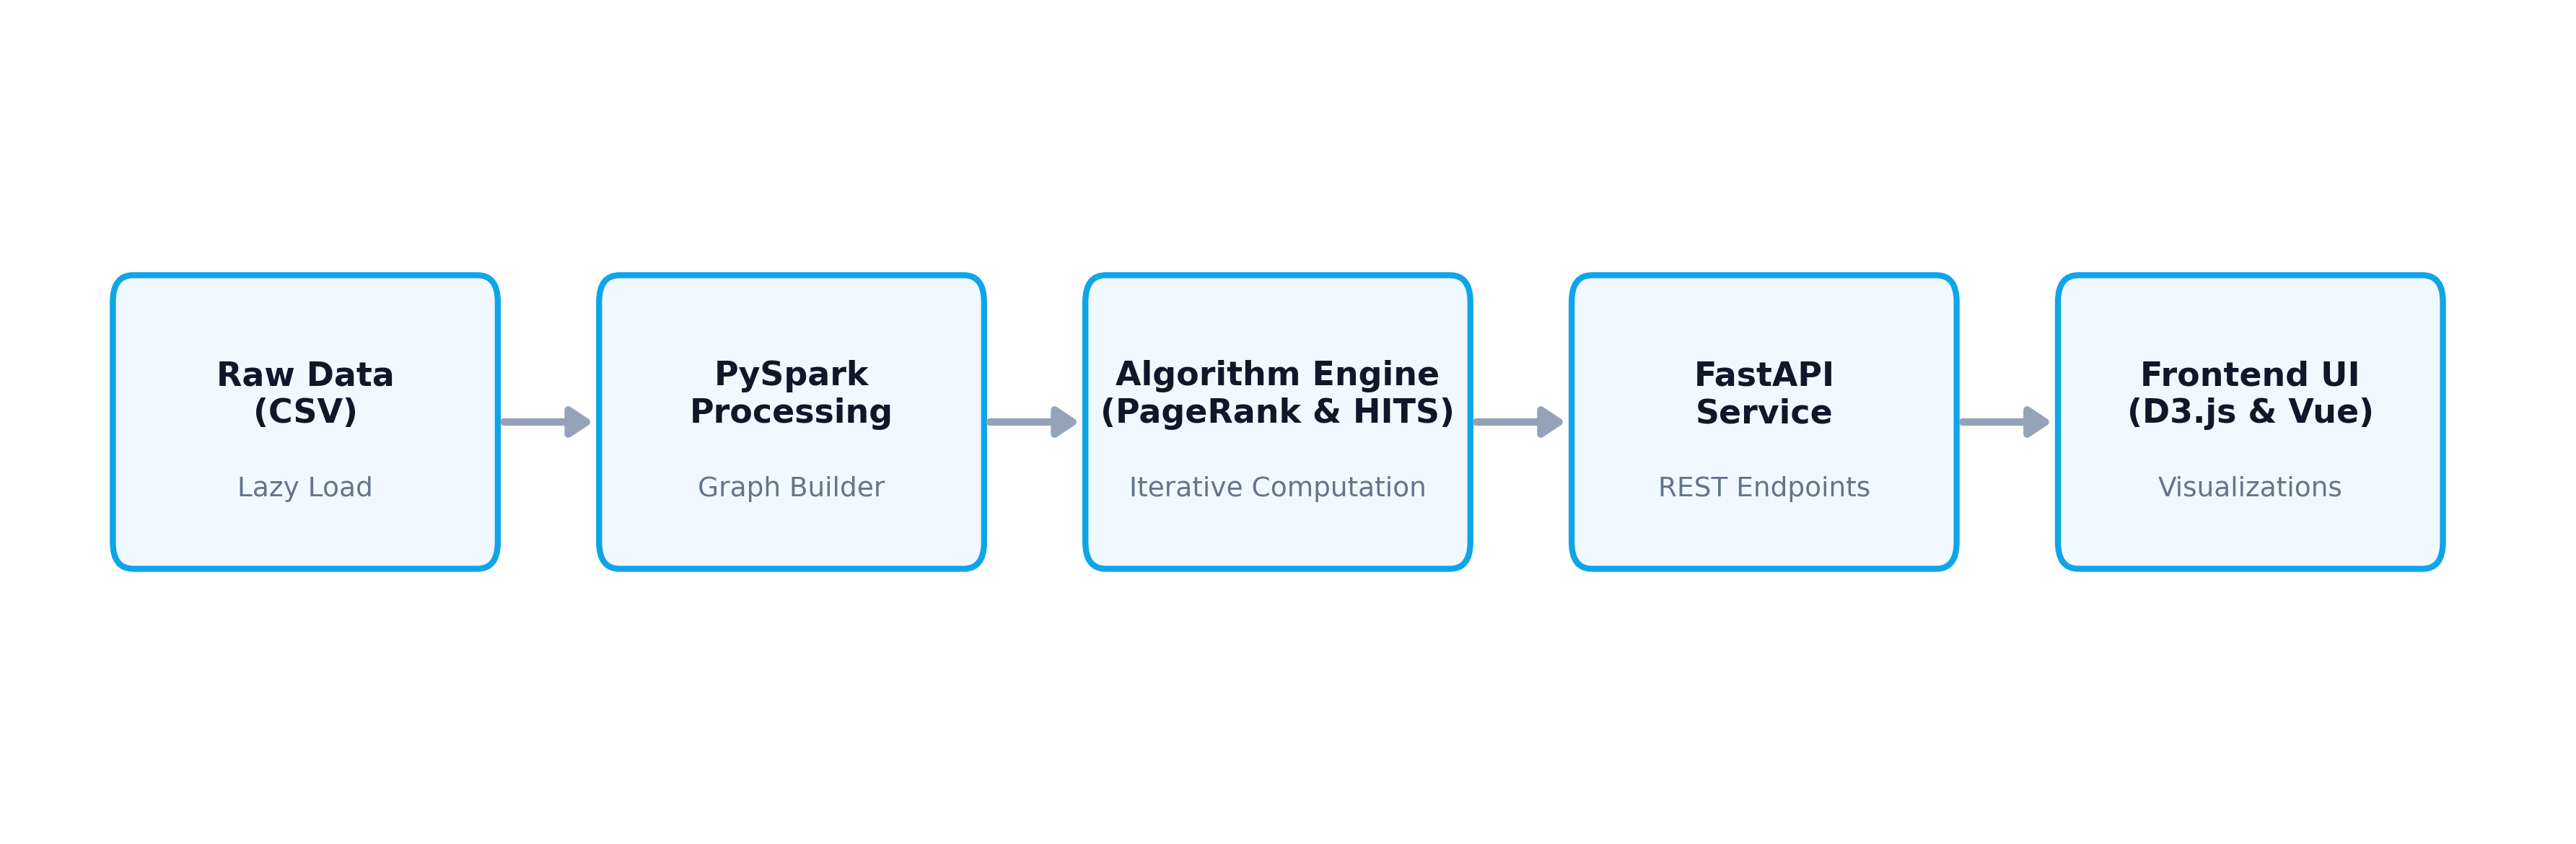
\includegraphics[width=0.9\textwidth]{Figures/system_workflow.png}
    \caption{Step-by-step system architecture workflow diagram of the Transfer Analyzer pipeline.}
    \label{fig:system_workflow}
\end{figure}


%=============================================================
\section{Transfer Analyzer Web Application}
\label{sec:transfer_analyzer}

The \textit{Transfer Analyzer} serves as the user-facing artifact of the thesis. It is not merely a visualization add-on, but an essential part of the methodology because it makes the comparison operational, reproducible, and inspectable by an end user.

\subsection{Backend Processing Workflow}
\label{subsec:backend_workflow}

When the application starts, a Spark session is initialized and the transfer dataset is preloaded into memory. For each incoming analysis request, the backend:
\begin{enumerate}
    \item reads the selected filters and algorithm parameters;
    \item builds the filtered transfer graph;
    \item executes the requested algorithm;
    \item extracts the top-ranked clubs and relevant edges;
    \item returns a structured JSON response containing node data, edge data, and metadata.
\end{enumerate}

Additional backend endpoints support league retrieval, transfer-detail lookup for specific clubs, historical ranking generation, and league-to-league flow computation.

\subsection{Frontend Analytical Views}
\label{subsec:frontend_views}

The frontend provides multiple complementary views of the same analytical output:
\begin{itemize}
    \item \textbf{Bar chart view:} emphasizes ranking order and score magnitude.
    \item \textbf{Network graph view:} emphasizes structural relationships among top-ranked clubs.
    \item \textbf{Flow view:} aggregates transfers at the league level to reveal broader movement patterns.
    \item \textbf{Compare mode:} renders PageRank and HITS side by side under identical filter settings.
    \item \textbf{Historical race chart:} animates the top-ranked clubs over time, featuring dynamic on-the-fly algorithm switching to instantly contrast PageRank and HITS on any given year.
\end{itemize}

The coexistence of these views is methodologically useful because no single visualization fully captures all aspects of graph behavior. Ranked bars show magnitude clearly, network layouts show relations, and animations expose temporal change.


%=============================================================
\section{Configurable Parameters}
\label{sec:configurable_params}

To ensure that the study is exploratory as well as comparative, the system exposes several parameters to the user:

\begin{itemize}
    \item \textbf{Algorithm:} PageRank or HITS;
    \item \textbf{Target direction:} buyers or sellers;
    \item \textbf{Iterations:} the number of update steps performed;
    \item \textbf{Damping factor:} applicable to PageRank;
    \item \textbf{Top-\emph{N}:} the number of clubs retained for visualization;
    \item \textbf{League filter:} limits analysis to a specific intra-league context;
    \item \textbf{Season range:} limits analysis to a selected temporal interval;
    \item \textbf{Weight mode:} fee-based or count-based edge weights.
\end{itemize}

This parameterization is essential for the thesis because it enables controlled comparisons. For example, changing only the weighting mode while keeping all other settings fixed provides insight into whether a club's prominence is driven by high-value transfers or by frequent transfer activity.


%=============================================================
\section{Algorithm Integration}
\label{sec:integration}

Both PageRank and HITS are implemented within the same processing framework and operate on the same aggregated edge representation.

\subsection{PageRank Integration}
\label{subsec:pagerank_integration}

PageRank is implemented as an iterative weighted propagation process over outgoing edges. For a node $u$ with outgoing neighbors $v$, the current rank of $u$ is distributed proportionally according to the normalized edge weights. The update rule used in the implementation is:
\[
PR_{t+1}(v) = (1-d) + d \sum_{u \in B(v)} PR_t(u) \cdot \frac{W(u,v)}{\sum_{x \in F(u)} W(u,x)}.
\]

This formulation preserves the spirit of weighted PageRank while adapting it to the football transfer network. A high rank is therefore assigned to clubs that receive transfers from already influential sellers.

\subsection{HITS Integration}
\label{subsec:hits_integration}

HITS is implemented on the same directed graph without reversing the edge direction. Starting from uniform initialization, the algorithm alternates between:
\begin{enumerate}
    \item updating authority scores from incoming hub contributions;
    \item normalizing authority scores;
    \item updating hub scores from outgoing authority contributions;
    \item normalizing hub scores.
\end{enumerate}

The update rules are:
\[
a(v) = \sum_{u:(u,v)\in E} h(u)\,W(u,v)
\]
and
\[
h(u) = \sum_{v:(u,v)\in E} a(v)\,W(u,v).
\]

The resulting authority and hub vectors reveal structurally different roles that are not captured by PageRank's single scalar score.

\subsection{Unified Comparison Logic}
\label{subsec:unified_comparison_logic}

The unified design of the system ensures that:
\begin{itemize}
    \item both algorithms use the same filtered dataset;
    \item both algorithms use the same graph construction process;
    \item both algorithms are exposed through the same service interface;
    \item both algorithms can be visualized individually or side by side.
\end{itemize}

This integration is fundamental to the thesis contribution because it transforms the comparison from a conceptual discussion into a reproducible computational experiment.


%=============================================================
\section{Expected Analytical Outputs}
\label{sec:expected_outputs}

The methodology is designed to produce several forms of output, each serving a distinct analytical purpose:

\begin{enumerate}
    \item \textbf{Club rankings:} top-$N$ lists of clubs ordered by PageRank, authority score, or hub score.
    \item \textbf{Score-aware network graphs:} club interaction networks annotated by computed score values.
    \item \textbf{Transfer detail panels:} club-specific summaries of important incoming and outgoing transfers.
    \item \textbf{League flow summaries:} aggregated movement between leagues.
    \item \textbf{Historical ranking timelines:} season-wise ranking sequences that reveal temporal evolution.
    \item \textbf{Comparative insights:} agreement and divergence between PageRank and HITS under matched configurations.
\end{enumerate}

These outputs are subsequently interpreted in the Results chapter to answer the research questions stated in Chapter~\ref{ch:introduction}. In particular, they enable the thesis to distinguish between globally central clubs, authority-like destination clubs, and hub-like supplier clubs, while also showing how these roles change across time, leagues, and weighting schemes.

